\PassOptionsToPackage{unicode=true}{hyperref} % options for packages loaded elsewhere
\PassOptionsToPackage{hyphens}{url}
%
\documentclass[12pt,]{article}
\usepackage{lmodern}
\usepackage{amssymb,amsmath}
\usepackage{ifxetex,ifluatex}
\usepackage{fixltx2e} % provides \textsubscript
\ifnum 0\ifxetex 1\fi\ifluatex 1\fi=0 % if pdftex
  \usepackage[T1]{fontenc}
  \usepackage[utf8]{inputenc}
  \usepackage{textcomp} % provides euro and other symbols
\else % if luatex or xelatex
  \usepackage{unicode-math}
  \defaultfontfeatures{Ligatures=TeX,Scale=MatchLowercase}
    \setmainfont[]{Times New Roman}
\fi
% use upquote if available, for straight quotes in verbatim environments
\IfFileExists{upquote.sty}{\usepackage{upquote}}{}
% use microtype if available
\IfFileExists{microtype.sty}{%
\usepackage[]{microtype}
\UseMicrotypeSet[protrusion]{basicmath} % disable protrusion for tt fonts
}{}
\IfFileExists{parskip.sty}{%
\usepackage{parskip}
}{% else
\setlength{\parindent}{0pt}
\setlength{\parskip}{6pt plus 2pt minus 1pt}
}
\usepackage{hyperref}
\hypersetup{
            pdftitle={Factors Influencing Above Ground Biomass of Forest Plots in the Congo},
            pdfauthor={Nikki Egna},
            pdfborder={0 0 0},
            breaklinks=true}
\urlstyle{same}  % don't use monospace font for urls
\usepackage[margin=2.54cm]{geometry}
\usepackage{color}
\usepackage{fancyvrb}
\newcommand{\VerbBar}{|}
\newcommand{\VERB}{\Verb[commandchars=\\\{\}]}
\DefineVerbatimEnvironment{Highlighting}{Verbatim}{commandchars=\\\{\}}
% Add ',fontsize=\small' for more characters per line
\usepackage{framed}
\definecolor{shadecolor}{RGB}{248,248,248}
\newenvironment{Shaded}{\begin{snugshade}}{\end{snugshade}}
\newcommand{\AlertTok}[1]{\textcolor[rgb]{0.94,0.16,0.16}{#1}}
\newcommand{\AnnotationTok}[1]{\textcolor[rgb]{0.56,0.35,0.01}{\textbf{\textit{#1}}}}
\newcommand{\AttributeTok}[1]{\textcolor[rgb]{0.77,0.63,0.00}{#1}}
\newcommand{\BaseNTok}[1]{\textcolor[rgb]{0.00,0.00,0.81}{#1}}
\newcommand{\BuiltInTok}[1]{#1}
\newcommand{\CharTok}[1]{\textcolor[rgb]{0.31,0.60,0.02}{#1}}
\newcommand{\CommentTok}[1]{\textcolor[rgb]{0.56,0.35,0.01}{\textit{#1}}}
\newcommand{\CommentVarTok}[1]{\textcolor[rgb]{0.56,0.35,0.01}{\textbf{\textit{#1}}}}
\newcommand{\ConstantTok}[1]{\textcolor[rgb]{0.00,0.00,0.00}{#1}}
\newcommand{\ControlFlowTok}[1]{\textcolor[rgb]{0.13,0.29,0.53}{\textbf{#1}}}
\newcommand{\DataTypeTok}[1]{\textcolor[rgb]{0.13,0.29,0.53}{#1}}
\newcommand{\DecValTok}[1]{\textcolor[rgb]{0.00,0.00,0.81}{#1}}
\newcommand{\DocumentationTok}[1]{\textcolor[rgb]{0.56,0.35,0.01}{\textbf{\textit{#1}}}}
\newcommand{\ErrorTok}[1]{\textcolor[rgb]{0.64,0.00,0.00}{\textbf{#1}}}
\newcommand{\ExtensionTok}[1]{#1}
\newcommand{\FloatTok}[1]{\textcolor[rgb]{0.00,0.00,0.81}{#1}}
\newcommand{\FunctionTok}[1]{\textcolor[rgb]{0.00,0.00,0.00}{#1}}
\newcommand{\ImportTok}[1]{#1}
\newcommand{\InformationTok}[1]{\textcolor[rgb]{0.56,0.35,0.01}{\textbf{\textit{#1}}}}
\newcommand{\KeywordTok}[1]{\textcolor[rgb]{0.13,0.29,0.53}{\textbf{#1}}}
\newcommand{\NormalTok}[1]{#1}
\newcommand{\OperatorTok}[1]{\textcolor[rgb]{0.81,0.36,0.00}{\textbf{#1}}}
\newcommand{\OtherTok}[1]{\textcolor[rgb]{0.56,0.35,0.01}{#1}}
\newcommand{\PreprocessorTok}[1]{\textcolor[rgb]{0.56,0.35,0.01}{\textit{#1}}}
\newcommand{\RegionMarkerTok}[1]{#1}
\newcommand{\SpecialCharTok}[1]{\textcolor[rgb]{0.00,0.00,0.00}{#1}}
\newcommand{\SpecialStringTok}[1]{\textcolor[rgb]{0.31,0.60,0.02}{#1}}
\newcommand{\StringTok}[1]{\textcolor[rgb]{0.31,0.60,0.02}{#1}}
\newcommand{\VariableTok}[1]{\textcolor[rgb]{0.00,0.00,0.00}{#1}}
\newcommand{\VerbatimStringTok}[1]{\textcolor[rgb]{0.31,0.60,0.02}{#1}}
\newcommand{\WarningTok}[1]{\textcolor[rgb]{0.56,0.35,0.01}{\textbf{\textit{#1}}}}
\usepackage{longtable,booktabs}
% Fix footnotes in tables (requires footnote package)
\IfFileExists{footnote.sty}{\usepackage{footnote}\makesavenoteenv{longtable}}{}
\usepackage{graphicx,grffile}
\makeatletter
\def\maxwidth{\ifdim\Gin@nat@width>\linewidth\linewidth\else\Gin@nat@width\fi}
\def\maxheight{\ifdim\Gin@nat@height>\textheight\textheight\else\Gin@nat@height\fi}
\makeatother
% Scale images if necessary, so that they will not overflow the page
% margins by default, and it is still possible to overwrite the defaults
% using explicit options in \includegraphics[width, height, ...]{}
\setkeys{Gin}{width=\maxwidth,height=\maxheight,keepaspectratio}
\setlength{\emergencystretch}{3em}  % prevent overfull lines
\providecommand{\tightlist}{%
  \setlength{\itemsep}{0pt}\setlength{\parskip}{0pt}}
\setcounter{secnumdepth}{5}
% Redefines (sub)paragraphs to behave more like sections
\ifx\paragraph\undefined\else
\let\oldparagraph\paragraph
\renewcommand{\paragraph}[1]{\oldparagraph{#1}\mbox{}}
\fi
\ifx\subparagraph\undefined\else
\let\oldsubparagraph\subparagraph
\renewcommand{\subparagraph}[1]{\oldsubparagraph{#1}\mbox{}}
\fi

% set default figure placement to htbp
\makeatletter
\def\fps@figure{htbp}
\makeatother

\usepackage{etoolbox}
\makeatletter
\providecommand{\subtitle}[1]{% add subtitle to \maketitle
  \apptocmd{\@title}{\par {\large #1 \par}}{}{}
}
\makeatother

\title{Factors Influencing Above Ground Biomass of Forest Plots in the Congo}
\providecommand{\subtitle}[1]{}
\subtitle{\url{https://github.com/nikki-egna/ENV872_Final_Project_Congo_Carbon}}
\author{Nikki Egna}
\date{}

\begin{document}
\maketitle

\newpage
\tableofcontents 
\newpage
\listoffigures

\newpage

\hypertarget{rationale-and-research-questions}{%
\section{Rationale and Research
Questions}\label{rationale-and-research-questions}}

Above ground biomass (AGB) is all biomass above the soil, including
woody and herbaceous vegetation, stems, stumps, branches, bark, and
foliage. Above ground biomass can be a predictor of overall health of a
forest ecosystem. It is also important for looking at carbon storage
potential of forests, which has significant implications for climate
change mitigation. (Ducanson et al., 2019) Researchers in forestry,
ecology, and agriculture often adopt the ``plot method'' for studying
AGB by estimating and monitoring production or changes in carbon stocks.
(Ducanson et al., 2019) The study conducted by the Poulsen Tropical
Ecology Lab utilizes this ``plot method'' to estimate AGB from plots in
the Republic of Congo, Africa. The Poulsen Lab estimated AGB using
methodology from Chave et al. (2014). This study utilizes these AGB
estimates to look at various environmental factors (covariates), and how
they might contribute to differences in AGB at each forest plot. The
environmental factors included in this study are Human Footprint Index
(HFI), GlobCover, annual precipitation, soil type, distance from the
nearest road, distance from the nearest village, distance from the
nearest river, distance from the nearest saw mill, and distance from the
nearest protected area. This study also quantifies the change in AGB
between the measurement collection years of 2005, 2009, and 2013.

\textbf{Question 1:}

How has above ground biomass changed over time at the plot locations?

\textbf{Question 2:}

Which environmental factors are signicant predictors of above ground
biomass?

\newpage

\hypertarget{dataset-information}{%
\section{Dataset Information}\label{dataset-information}}

This repository uses data from the Poulsen Tropical Ecology Lab, and
contains information on tree diameter and species from plots in the
Congo. This data is being collected in order to model the amount of
above ground biomass (AGB) within each plot across the study sites.
Utilizing remote sensing techniques, the Poulsen Lab performed analysis
to determine several covariate values at each plot, including distance
to nearest road, distance to nearest village, distance to nearest river,
distance to nearest protected area, Human Footprint Index, and Globcover
value. This project will look at which covariates have a significant
impact on AGB at the study sites.

The CongoCarbon\_Raw\_Data.csv was collected by the Poulsen Tropical
Ecology Lab, and their on-ground team based in the Congo. This data is
not public facing, and access was granted through Dr.~John Poulsen. The
CongoCarbon\_AGB\_by\_Plot.csv was created by John Poulsen, Anna
Nordseth, and Nikki Egna based on the raw data. The covariate data
(CongoCarbon\_Plot\_Covariates.csv) was created by Nikki Egna in March
of 2020, and the data it utilizes was obtained from the following
sources: Human Footprint Index was derived from Wildlife Conservation
Society (WCS), Center for International Earth Science Information
Network (CIESIN), and Columbia University and was accessed in December
of 2019. The GlobCover raster was downloaded from the ESA Globcover 2005
Project, led by MEDIAS-France/POSTEL, in December of 2019. Precipitation
data was obtained from the Climate Hazards group Infrared Precipitation
with Stations (CHIRPS) in December of 2019. The roads, river, soil, saw
mill, and villages data comes from the Ministère de l'Économie
Forestière CNIAF\_MEFDD (\url{https://cog.forest-atlas.org}), accessed
in April, 2020.

\hypertarget{metadata}{%
\subsection{Metadata}\label{metadata}}

\hypertarget{congocarbon_raw_data.csv}{%
\subsubsection{CongoCarbon\_Raw\_data.csv}\label{congocarbon_raw_data.csv}}

\begin{longtable}[]{@{}ll@{}}
\toprule
Column Name & Description\tabularnewline
\midrule
\endhead
Tree ID & Identification number assigned to the unique tree
(Numeric)\tabularnewline
Tag No & Secondary tree identification number (Numeric)\tabularnewline
Plot & Study plot number (Numeric)\tabularnewline
Subplot & Subplot number within each plot (Numeric)\tabularnewline
Family & Tree family name (Character)\tabularnewline
Species & Tree species name (Character)\tabularnewline
WD & Wood density (Numeric)\tabularnewline
DBH0\_05 & First diameter measurement in 2005 (Numeric;
Centimeters)\tabularnewline
DBH1\_05 & Second diameter measurement in 2005 (Numeric;
Centimeters)\tabularnewline
DBH2\_05 & Third diameter measurement in 2005 (Numeric;
Centimeters)\tabularnewline
DBH3\_05 & Fourth diameter measurement in 2005 (Numeric;
Centimeters)\tabularnewline
DBH4\_05 & Fifth diameter measurement in 2005 (Numeric;
Centimeters)\tabularnewline
DBH0\_09 & First diameter measurement in 2009 (Numeric;
Centimeters)\tabularnewline
DBH1\_09 & Second diameter measurement in 2009 (Numeric;
Centimeters)\tabularnewline
DBH2\_09 & Third diameter measurement in 2009 (Numeric;
Centimeters)\tabularnewline
DBH3\_09 & Fourth diameter measurement in 2009 (Numeric;
Centimeters)\tabularnewline
DBH4\_09 & Fifth diameter measurement in 2009 (Numeric;
Centimeters)\tabularnewline
DBH0\_13 & First diameter measurement in 2013 (Numeric;
Centimeters)\tabularnewline
DBH1\_13 & Second diameter measurement in 2013 (Numeric;
Centimeters)\tabularnewline
DBH2\_13 & Third diameter measurement in 2013 (Numeric;
Centimeters)\tabularnewline
DBH3\_13 & Fourth diameter measurement in 2013 (Numeric;
Centimeters)\tabularnewline
DBH4\_13 & Fifth diameter measurement in 2013 (Numeric;
Centimeters)\tabularnewline
AGB05.MgE & AGB estimate 2005 (Numeric; milligrams)\tabularnewline
AGB09.MgE & AGB estimate 2009 (Numeric; milligrams)\tabularnewline
AGB13.MgE & AGB estimate 2013 (Numeric; milligrams)\tabularnewline
\bottomrule
\end{longtable}

\hypertarget{congocarbon_plot_covariates.csv}{%
\subsubsection{CongoCarbon\_Plot\_Covariates.csv}\label{congocarbon_plot_covariates.csv}}

\begin{longtable}[]{@{}ll@{}}
\toprule
\begin{minipage}[b]{0.53\columnwidth}\raggedright
Column Name\strut
\end{minipage} & \begin{minipage}[b]{0.41\columnwidth}\raggedright
Description\strut
\end{minipage}\tabularnewline
\midrule
\endhead
\begin{minipage}[t]{0.53\columnwidth}\raggedright
Plot\strut
\end{minipage} & \begin{minipage}[t]{0.41\columnwidth}\raggedright
Tree plot ID number (Factor)\strut
\end{minipage}\tabularnewline
\begin{minipage}[t]{0.53\columnwidth}\raggedright
Latitude\strut
\end{minipage} & \begin{minipage}[t]{0.41\columnwidth}\raggedright
Latitude of the plot (Numeric)\strut
\end{minipage}\tabularnewline
\begin{minipage}[t]{0.53\columnwidth}\raggedright
Longitude\strut
\end{minipage} & \begin{minipage}[t]{0.41\columnwidth}\raggedright
Longitude of the plot (Numeric)\strut
\end{minipage}\tabularnewline
\begin{minipage}[t]{0.53\columnwidth}\raggedright
HFI\strut
\end{minipage} & \begin{minipage}[t]{0.41\columnwidth}\raggedright
Human Footprint Index value at the plot location (Factor)\strut
\end{minipage}\tabularnewline
\begin{minipage}[t]{0.53\columnwidth}\raggedright
GlobCover\strut
\end{minipage} & \begin{minipage}[t]{0.41\columnwidth}\raggedright
GlobCover vegetation index value at the plot location (Factor)\strut
\end{minipage}\tabularnewline
\begin{minipage}[t]{0.53\columnwidth}\raggedright
Precip\_sum\_2013\strut
\end{minipage} & \begin{minipage}[t]{0.41\columnwidth}\raggedright
Annual precipitation sum for 2013 at plot location (Numeric;
millimeters)\strut
\end{minipage}\tabularnewline
\begin{minipage}[t]{0.53\columnwidth}\raggedright
Soil\strut
\end{minipage} & \begin{minipage}[t]{0.41\columnwidth}\raggedright
Soil type index at plot location (Factor)\strut
\end{minipage}\tabularnewline
\begin{minipage}[t]{0.53\columnwidth}\raggedright
Dist\_Road\_m\strut
\end{minipage} & \begin{minipage}[t]{0.41\columnwidth}\raggedright
Distance from plot to the nearest road (Numeric; Meters)\strut
\end{minipage}\tabularnewline
\begin{minipage}[t]{0.53\columnwidth}\raggedright
Dist\_Village\_m\strut
\end{minipage} & \begin{minipage}[t]{0.41\columnwidth}\raggedright
Distance from plot to the nearest village (Numeric; Meters)\strut
\end{minipage}\tabularnewline
\begin{minipage}[t]{0.53\columnwidth}\raggedright
Dist\_River\_m\strut
\end{minipage} & \begin{minipage}[t]{0.41\columnwidth}\raggedright
Distance from plot to the nearest river (Numeric; Meters)\strut
\end{minipage}\tabularnewline
\begin{minipage}[t]{0.53\columnwidth}\raggedright
Dist\_PA\_m\strut
\end{minipage} & \begin{minipage}[t]{0.41\columnwidth}\raggedright
Distance from plot to the nearest protected area (Numeric; Meters)\strut
\end{minipage}\tabularnewline
\begin{minipage}[t]{0.53\columnwidth}\raggedright
Dist\_Saw\_Mills\_m\strut
\end{minipage} & \begin{minipage}[t]{0.41\columnwidth}\raggedright
Distance from plot to the nearest saw mill (Numeric; Meters)\strut
\end{minipage}\tabularnewline
\bottomrule
\end{longtable}

\newpage

\hypertarget{exploratory-analysis}{%
\section{Exploratory Analysis}\label{exploratory-analysis}}

\hypertarget{raw-data}{%
\subsection{Raw Data}\label{raw-data}}

To explore the raw data, the first few rows and the structure of the
dataframe were analyzed. The class of each of the columns was also
assesed, and any incorrect column classes were corrected. For this
analysis, only the `Plot' column needed to be changed from numeric to a
factor variable. The number of empty rows within the AGB measurement
columns were also checked and quantified. It is critical to know if
there were any missing measurements. Approximately 10\% of the data had
missing values. The number of missing measurements, was reported back to
The Poulsen Tropical Ecology Lab. It should be noted that the presence
of missing data may alter the accuracy of the analysis presented here.

\begin{Shaded}
\begin{Highlighting}[]
\CommentTok{#Check first few rows of data and the structure of the data}
\KeywordTok{head}\NormalTok{(Raw_CongoCarbon_Data)}
\KeywordTok{str}\NormalTok{(Raw_CongoCarbon_Data)}

\CommentTok{#Check class of necessary columns}
\KeywordTok{lapply}\NormalTok{(Raw_CongoCarbon_Data, class)}

\CommentTok{#Change necessary classes}
\NormalTok{Raw_CongoCarbon_Data}\OperatorTok{$}\NormalTok{Plot <-}\StringTok{ }\KeywordTok{as.factor}\NormalTok{(Raw_CongoCarbon_Data}\OperatorTok{$}\NormalTok{Plot)}

\CommentTok{#Check for NAs}
\KeywordTok{anyNA}\NormalTok{(Raw_CongoCarbon_Data}\OperatorTok{$}\NormalTok{AGB05.MgE)}
\KeywordTok{anyNA}\NormalTok{(Raw_CongoCarbon_Data}\OperatorTok{$}\NormalTok{AGB09.MgE)}
\KeywordTok{anyNA}\NormalTok{(Raw_CongoCarbon_Data}\OperatorTok{$}\NormalTok{AGB13.MgE)}

\CommentTok{#Look at number of NA values}
\KeywordTok{nrow}\NormalTok{(}\KeywordTok{subset}\NormalTok{(Raw_CongoCarbon_Data, }\KeywordTok{is.na}\NormalTok{(AGB05.MgE)))}
\KeywordTok{nrow}\NormalTok{(}\KeywordTok{subset}\NormalTok{(Raw_CongoCarbon_Data, }\KeywordTok{is.na}\NormalTok{(AGB09.MgE)))}
\KeywordTok{nrow}\NormalTok{(}\KeywordTok{subset}\NormalTok{(Raw_CongoCarbon_Data, }\KeywordTok{is.na}\NormalTok{(AGB13.MgE)))}

\CommentTok{#Proportion of NAs }
\NormalTok{(}\KeywordTok{nrow}\NormalTok{(}\KeywordTok{subset}\NormalTok{(Raw_CongoCarbon_Data, }\KeywordTok{is.na}\NormalTok{(AGB05.MgE)))}\OperatorTok{/}\KeywordTok{nrow}\NormalTok{(Raw_CongoCarbon_Data))}\OperatorTok{*}\DecValTok{100}
\end{Highlighting}
\end{Shaded}

\hypertarget{covariate-data}{%
\subsection{Covariate Data}\label{covariate-data}}

The dataset containing the covariate values at each plot was analyzed
similarly to the raw data. The beginning rows of the dataset, as well as
the structure, and then the class of each column were assessed.

\begin{Shaded}
\begin{Highlighting}[]
\KeywordTok{head}\NormalTok{(CongoCarbon_Covariates)}
\KeywordTok{str}\NormalTok{(CongoCarbon_Covariates)}

\CommentTok{#Check the class for all columns in CongoCarbon_Covariates}
\KeywordTok{lapply}\NormalTok{(CongoCarbon_Covariates, class)}
\end{Highlighting}
\end{Shaded}

\hypertarget{analysis}{%
\section{Analysis}\label{analysis}}

The raw data was wrangled in order to obtain the AGB sum of all the
trees within each plot. Columns for the change in AGB between the years
were created by subtracting the sum AGB of the following measurement
year from the sum AGB from the prior measurement year. This created a
data frame (AGB\_by\_Plot) with the plot number and the total sum AGB at
each plot for the years 2005, 2009, and 2013, as well as the change in
AGB from 2005-2009, 2009-2013, and 2005-2013. The AGB\_by\_Plot data
from was then merged with the raw covariates data to create one final
dataframe. This final data frame includes plot number, all covariate
values at each plot, the sum AGB for each year at each plot, and the
change in AGB from one measurement year to another for each plot. This
data frame is saved as CongoCarbon\_AGB\_and\_Covariates\_by\_Plot.csv
in the Data/Processed directory of the repository.

\begin{Shaded}
\begin{Highlighting}[]
\CommentTok{#Create columns with the sum AGB by plot for each year '05, '09, '13}
\NormalTok{AGB_by_Plot <-}\StringTok{ }\NormalTok{Raw_CongoCarbon_Data }\OperatorTok
\StringTok{  }\KeywordTok{group_by}\NormalTok{(Plot) }\OperatorTok
\StringTok{  }\KeywordTok{summarize}\NormalTok{(}\DataTypeTok{sum_AGB05 =} \KeywordTok{sum}\NormalTok{(AGB05.MgE, }\DataTypeTok{na.rm =} \OtherTok{TRUE}\NormalTok{), }
            \DataTypeTok{sum_AGB09 =} \KeywordTok{sum}\NormalTok{(AGB09.MgE, }\DataTypeTok{na.rm =} \OtherTok{TRUE}\NormalTok{), }
            \DataTypeTok{sum_AGB13 =} \KeywordTok{sum}\NormalTok{(AGB13.MgE, }\DataTypeTok{na.rm =} \OtherTok{TRUE}\NormalTok{))}

\CommentTok{#Create columns for change in AGB from '05-'09, '09-'13, & '05-'13}
\NormalTok{AGB_by_Plot}\OperatorTok{$}\NormalTok{change0509 <-}\StringTok{ }\KeywordTok{with}\NormalTok{(AGB_by_Plot, sum_AGB09 }\OperatorTok{-}\StringTok{ }\NormalTok{sum_AGB05)}
\NormalTok{AGB_by_Plot}\OperatorTok{$}\NormalTok{change0913 <-}\StringTok{ }\KeywordTok{with}\NormalTok{(AGB_by_Plot, sum_AGB13 }\OperatorTok{-}\StringTok{ }\NormalTok{sum_AGB09)}
\NormalTok{AGB_by_Plot}\OperatorTok{$}\NormalTok{change0513 <-}\StringTok{ }\KeywordTok{with}\NormalTok{(AGB_by_Plot, sum_AGB13 }\OperatorTok{-}\StringTok{ }\NormalTok{sum_AGB05)}

\CommentTok{#Combine AGB_by_Plot and CongoCarbon_Covariates by plot}
\NormalTok{AGB_and_Covariates_by_Plot <-}\StringTok{ }
\StringTok{  }\KeywordTok{merge}\NormalTok{(CongoCarbon_Covariates, AGB_by_Plot, }\DataTypeTok{by=}\StringTok{"Plot"}\NormalTok{)}
\end{Highlighting}
\end{Shaded}

Further data wrangling was necessary in order to graph this data. The
dataframe created above (AGB\_and\_Covariates\_by\_Plot) is in
horizontal form. In order to move forward with this analysis, the data
must be in vertical form, so the melt() function was implemented to
complete this task. Through use of this tool, a new dataframe
(melted\_AGB\_by\_Plot) was created, containing columns for plot, year,
the variable (either sum AGB or change in AGB) and the AGB value. Rather
than having multiple columns for each measurement year of AGB and
multiple columns for the change in AGB measurements, there is now one
column for AGB value, one column for year, and one column for variable.
The melted dataframe was then subsetted to make two new sets of data,
one for the sum values of AGB, and one for the values of change in AGB.
The same process was applied to the original raw data
(Raw\_CongoCarbon\_data) by selecting the necessary columns and applying
the melt function.

\begin{Shaded}
\begin{Highlighting}[]
\CommentTok{#Change dataframe from horizontal to vertical}
\NormalTok{melted_AGB_by_Plot <-}\StringTok{ }\KeywordTok{melt}\NormalTok{(AGB_by_Plot, }\DataTypeTok{id=}\KeywordTok{c}\NormalTok{(}\StringTok{"Plot"}\NormalTok{))}
\CommentTok{#Create a column for year}
\NormalTok{melted_AGB_by_Plot}\OperatorTok{$}\NormalTok{Year <-}\StringTok{ }\NormalTok{melted_AGB_by_Plot}\OperatorTok{$}\NormalTok{variable}
\NormalTok{melted_AGB_by_Plot}\OperatorTok{$}\NormalTok{Year <-}\StringTok{ }\KeywordTok{gsub}\NormalTok{(}\StringTok{"sum_AGB05"}\NormalTok{,}\StringTok{"2005"}\NormalTok{, }
\NormalTok{                                melted_AGB_by_Plot}\OperatorTok{$}\NormalTok{Year, }\DataTypeTok{fixed=}\NormalTok{T)}
\NormalTok{melted_AGB_by_Plot}\OperatorTok{$}\NormalTok{Year <-}\StringTok{ }\KeywordTok{gsub}\NormalTok{(}\StringTok{"sum_AGB09"}\NormalTok{,}\StringTok{"2009"}\NormalTok{, }
\NormalTok{                                melted_AGB_by_Plot}\OperatorTok{$}\NormalTok{Year, }\DataTypeTok{fixed=}\NormalTok{T)}
\NormalTok{melted_AGB_by_Plot}\OperatorTok{$}\NormalTok{Year <-}\StringTok{ }\KeywordTok{gsub}\NormalTok{(}\StringTok{"sum_AGB13"}\NormalTok{,}\StringTok{"2013"}\NormalTok{, }
\NormalTok{                                melted_AGB_by_Plot}\OperatorTok{$}\NormalTok{Year, }\DataTypeTok{fixed=}\NormalTok{T)}

\CommentTok{#Create dataframe for the sum of AGB by plot}
\NormalTok{sum_AGB_by_plot <-}\StringTok{ }\NormalTok{melted_AGB_by_Plot[melted_AGB_by_Plot}\OperatorTok{$}\NormalTok{variable }
                                      \OperatorTok\StringTok{ "sum"}\NormalTok{, ]}
\CommentTok{#Create dataframe for the change in AGB by plot}
\NormalTok{change_AGB_by_plot <-}\StringTok{ }\NormalTok{melted_AGB_by_Plot[melted_AGB_by_Plot}\OperatorTok{$}\NormalTok{variable }
                                         \OperatorTok\StringTok{ "change"}\NormalTok{, ]}
\CommentTok{#Create dataframe for the change in AGB by year}
\NormalTok{AGB_change_by_year <-}\StringTok{ }\NormalTok{change_AGB_by_plot }\OperatorTok
\StringTok{  }\KeywordTok{group_by}\NormalTok{(variable) }\OperatorTok
\StringTok{  }\KeywordTok{summarise}\NormalTok{(}\DataTypeTok{sum=}\KeywordTok{sum}\NormalTok{(value))}

\CommentTok{#Subset necessary data}
\NormalTok{Raw_data_subset <-}\StringTok{ }\NormalTok{Raw_CongoCarbon_Data }\OperatorTok
\StringTok{  }\NormalTok{dplyr}\OperatorTok{::}\KeywordTok{select}\NormalTok{(Tree.ID, Plot, AGB05.MgE, AGB09.MgE, AGB13.MgE)}

\CommentTok{#Melt data}
\NormalTok{melted_raw_data <-}\StringTok{ }\KeywordTok{melt}\NormalTok{(Raw_data_subset, }\DataTypeTok{id=}\KeywordTok{c}\NormalTok{(}\StringTok{"Tree.ID"}\NormalTok{,}\StringTok{"Plot"}\NormalTok{))}

\CommentTok{#Create a column for year}
\NormalTok{melted_raw_data}\OperatorTok{$}\NormalTok{Year <-}\StringTok{ }\NormalTok{melted_raw_data}\OperatorTok{$}\NormalTok{variable}
\NormalTok{melted_raw_data}\OperatorTok{$}\NormalTok{Year <-}\StringTok{ }\KeywordTok{gsub}\NormalTok{(}\StringTok{"AGB05.MgE"}\NormalTok{,}\StringTok{"2005"}\NormalTok{, }
\NormalTok{                             melted_raw_data}\OperatorTok{$}\NormalTok{Year, }\DataTypeTok{fixed=}\NormalTok{T)}
\NormalTok{melted_raw_data}\OperatorTok{$}\NormalTok{Year <-}\StringTok{ }\KeywordTok{gsub}\NormalTok{(}\StringTok{"AGB09.MgE"}\NormalTok{,}\StringTok{"2009"}\NormalTok{, }
\NormalTok{                             melted_raw_data}\OperatorTok{$}\NormalTok{Year, }\DataTypeTok{fixed=}\NormalTok{T)}
\NormalTok{melted_raw_data}\OperatorTok{$}\NormalTok{Year <-}\StringTok{ }\KeywordTok{gsub}\NormalTok{(}\StringTok{"AGB13.MgE"}\NormalTok{,}\StringTok{"2013"}\NormalTok{, }
\NormalTok{                             melted_raw_data}\OperatorTok{$}\NormalTok{Year, }\DataTypeTok{fixed=}\NormalTok{T)}
\end{Highlighting}
\end{Shaded}

\newpage

\hypertarget{data-visualization}{%
\subsection{Data visualization}\label{data-visualization}}

Figure 1 shows histograms of the AGB values of the raw data for each
year. This provides general insight about the data, such as the
normality, whether there are outliers present, and also compares the
values of AGB measurements for each of the years. We can see that, for
all years, a vast majority of the measurements are very low (between 0
and 10 Mg), but there are a few significant outliers (Figure 1).

\begin{figure}
\centering
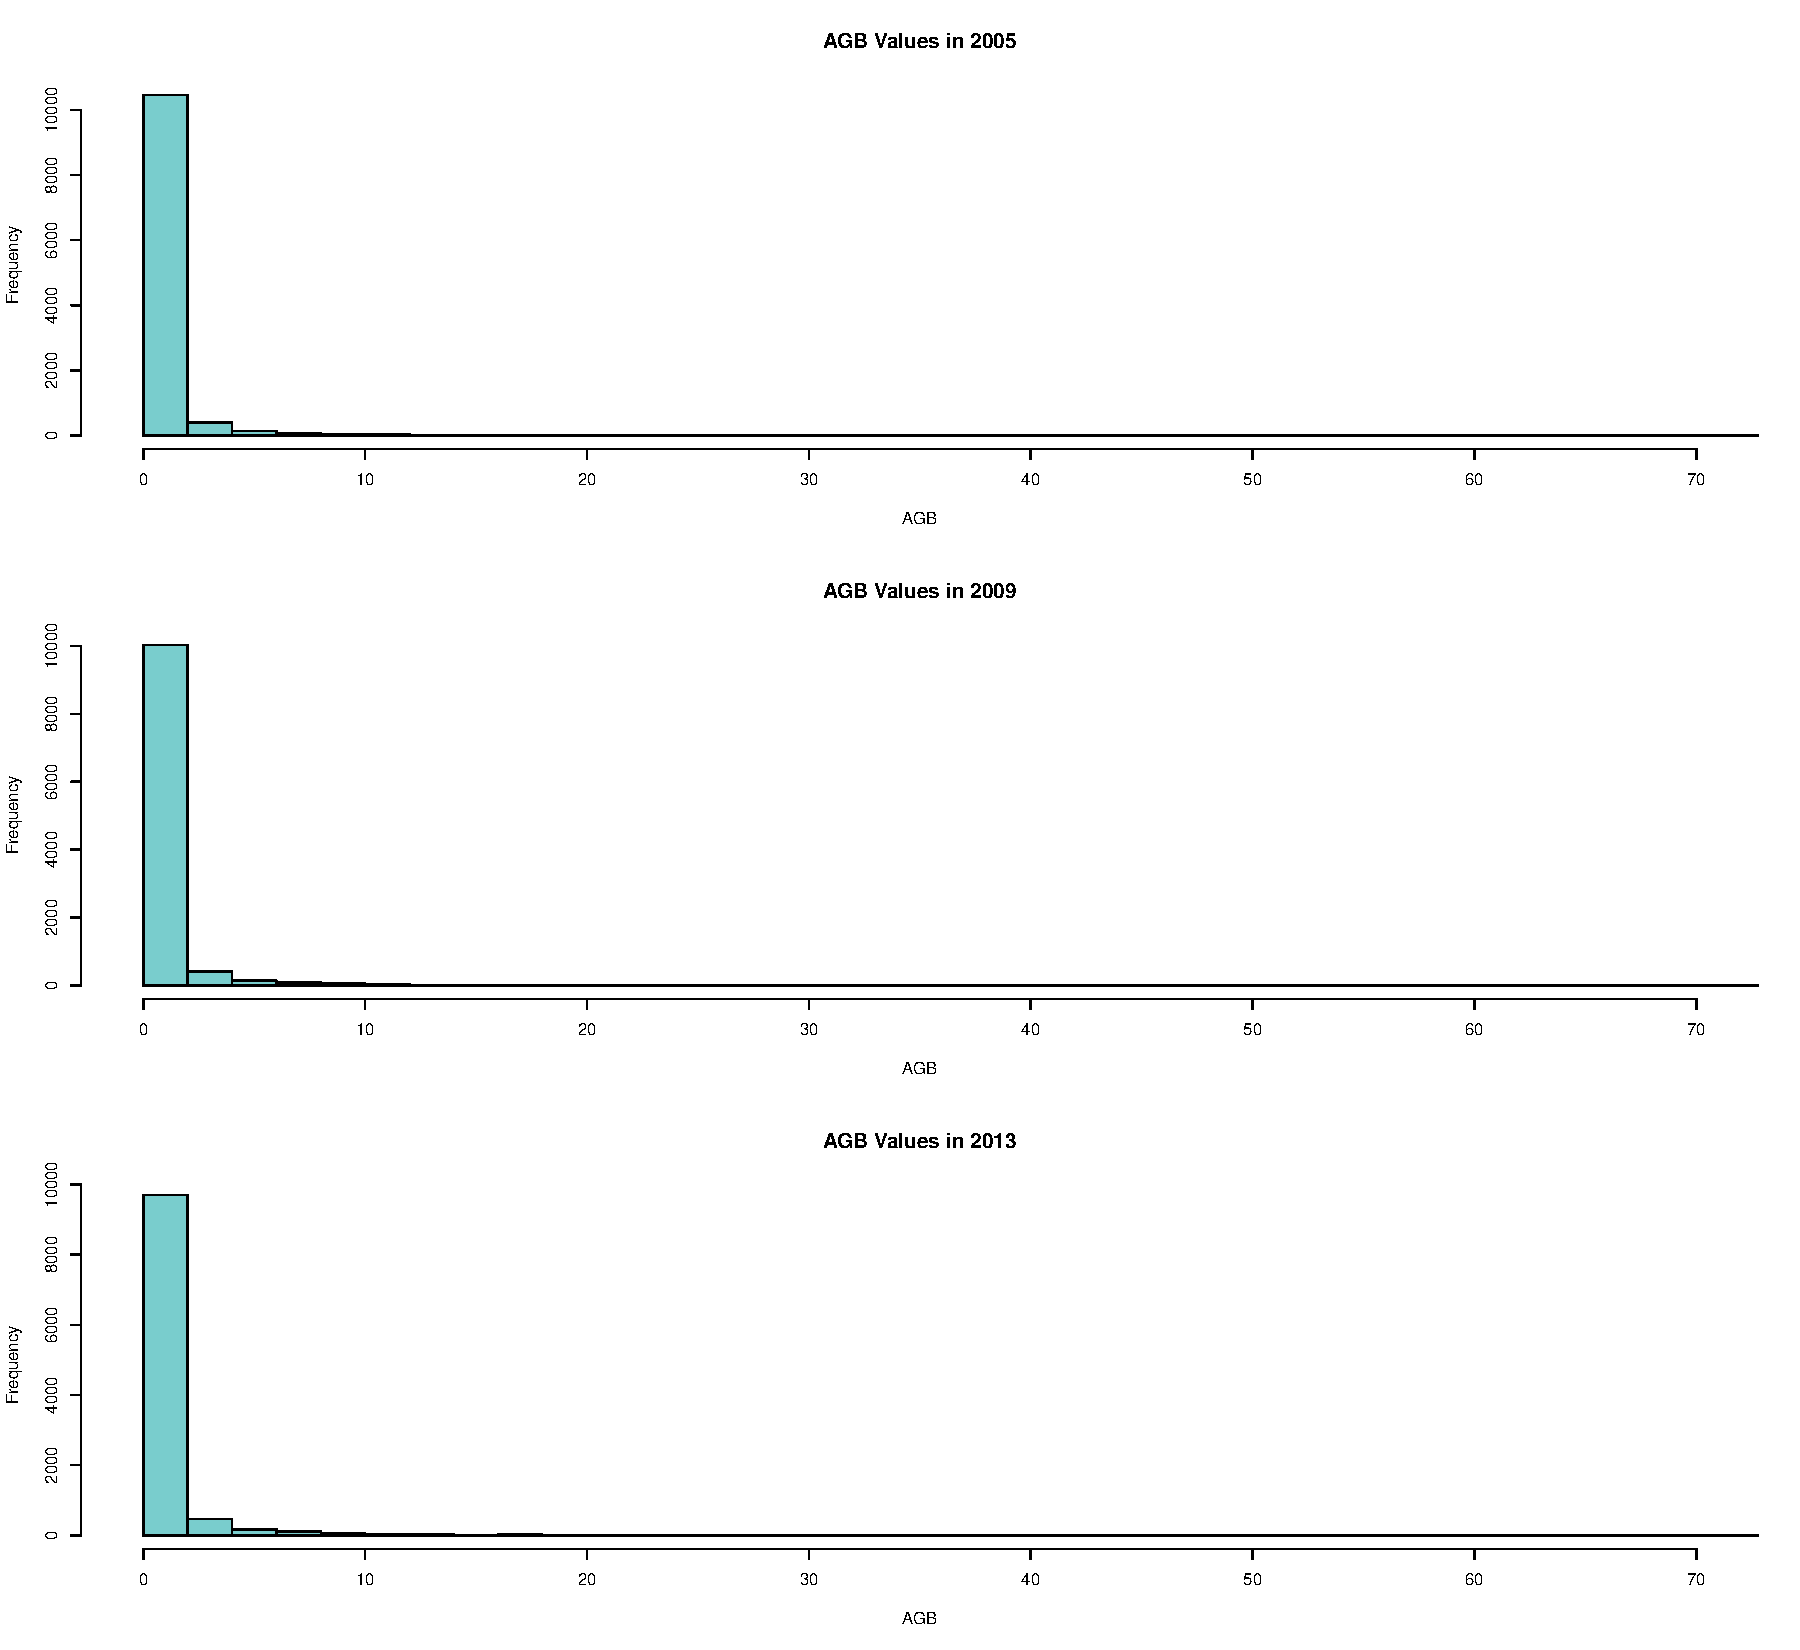
\includegraphics{Project_Template_files/figure-latex/histograms-1.pdf}
\caption{Histogram showing the distribution of AGB measurements of the
trees for 2005, 2009, and 2013.}
\end{figure}

\begin{verbatim}
## null device 
##           1
\end{verbatim}

\newpage

In order to further vizualize how AGB may differ between the
measurements years, a line graph represents the change in the sum of AGB
of each plot over time (Figure 2). Each line represents a different plot
number. Here, we can speculate that there was not much change in AGB
from 2005 to 2009, however there was significant change from 2009 to
2013.

\begin{figure}
\centering
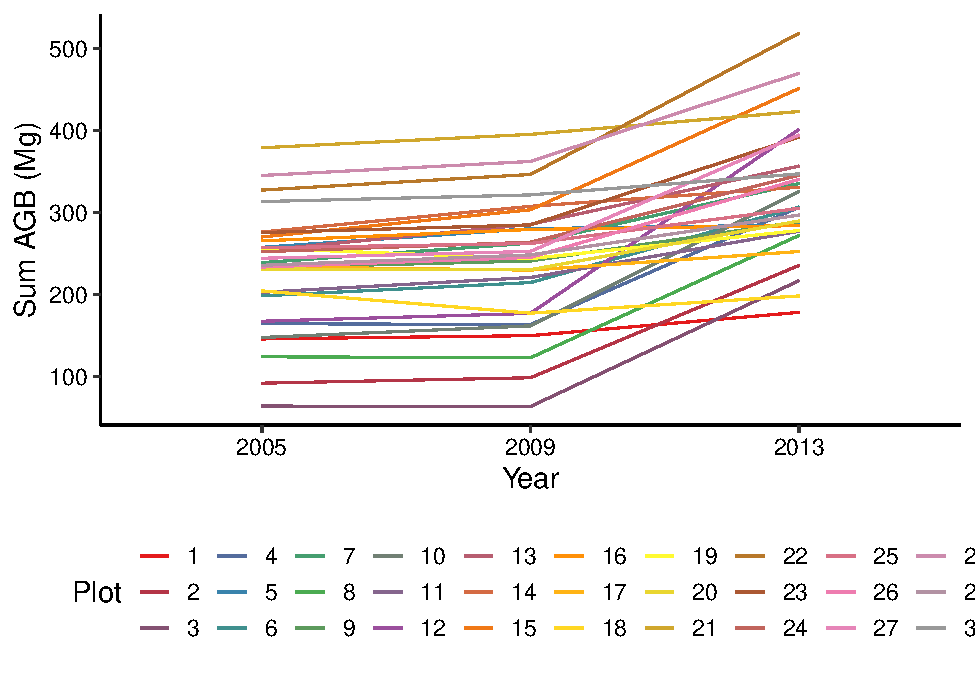
\includegraphics{Project_Template_files/figure-latex/data_visualization-1.pdf}
\caption{Relationship of the changes in total above ground biomass at
each plot between 2005, 2009, and 2013.}
\end{figure}

The following violin plot shows the distribution of AGB measurements
within each plot for 2005, 2009, and 2013 (Figure 3). Similar to the
histogram, we can see that a majority of the values are low
measurements, with the presence of significant outliers. We can see here
the differences in AGB values not only between the different trees
within each plots (shown by the long tails), however we also see that
there are differences between the overall sum AGB from one plot to
another.

\begin{figure}
\centering
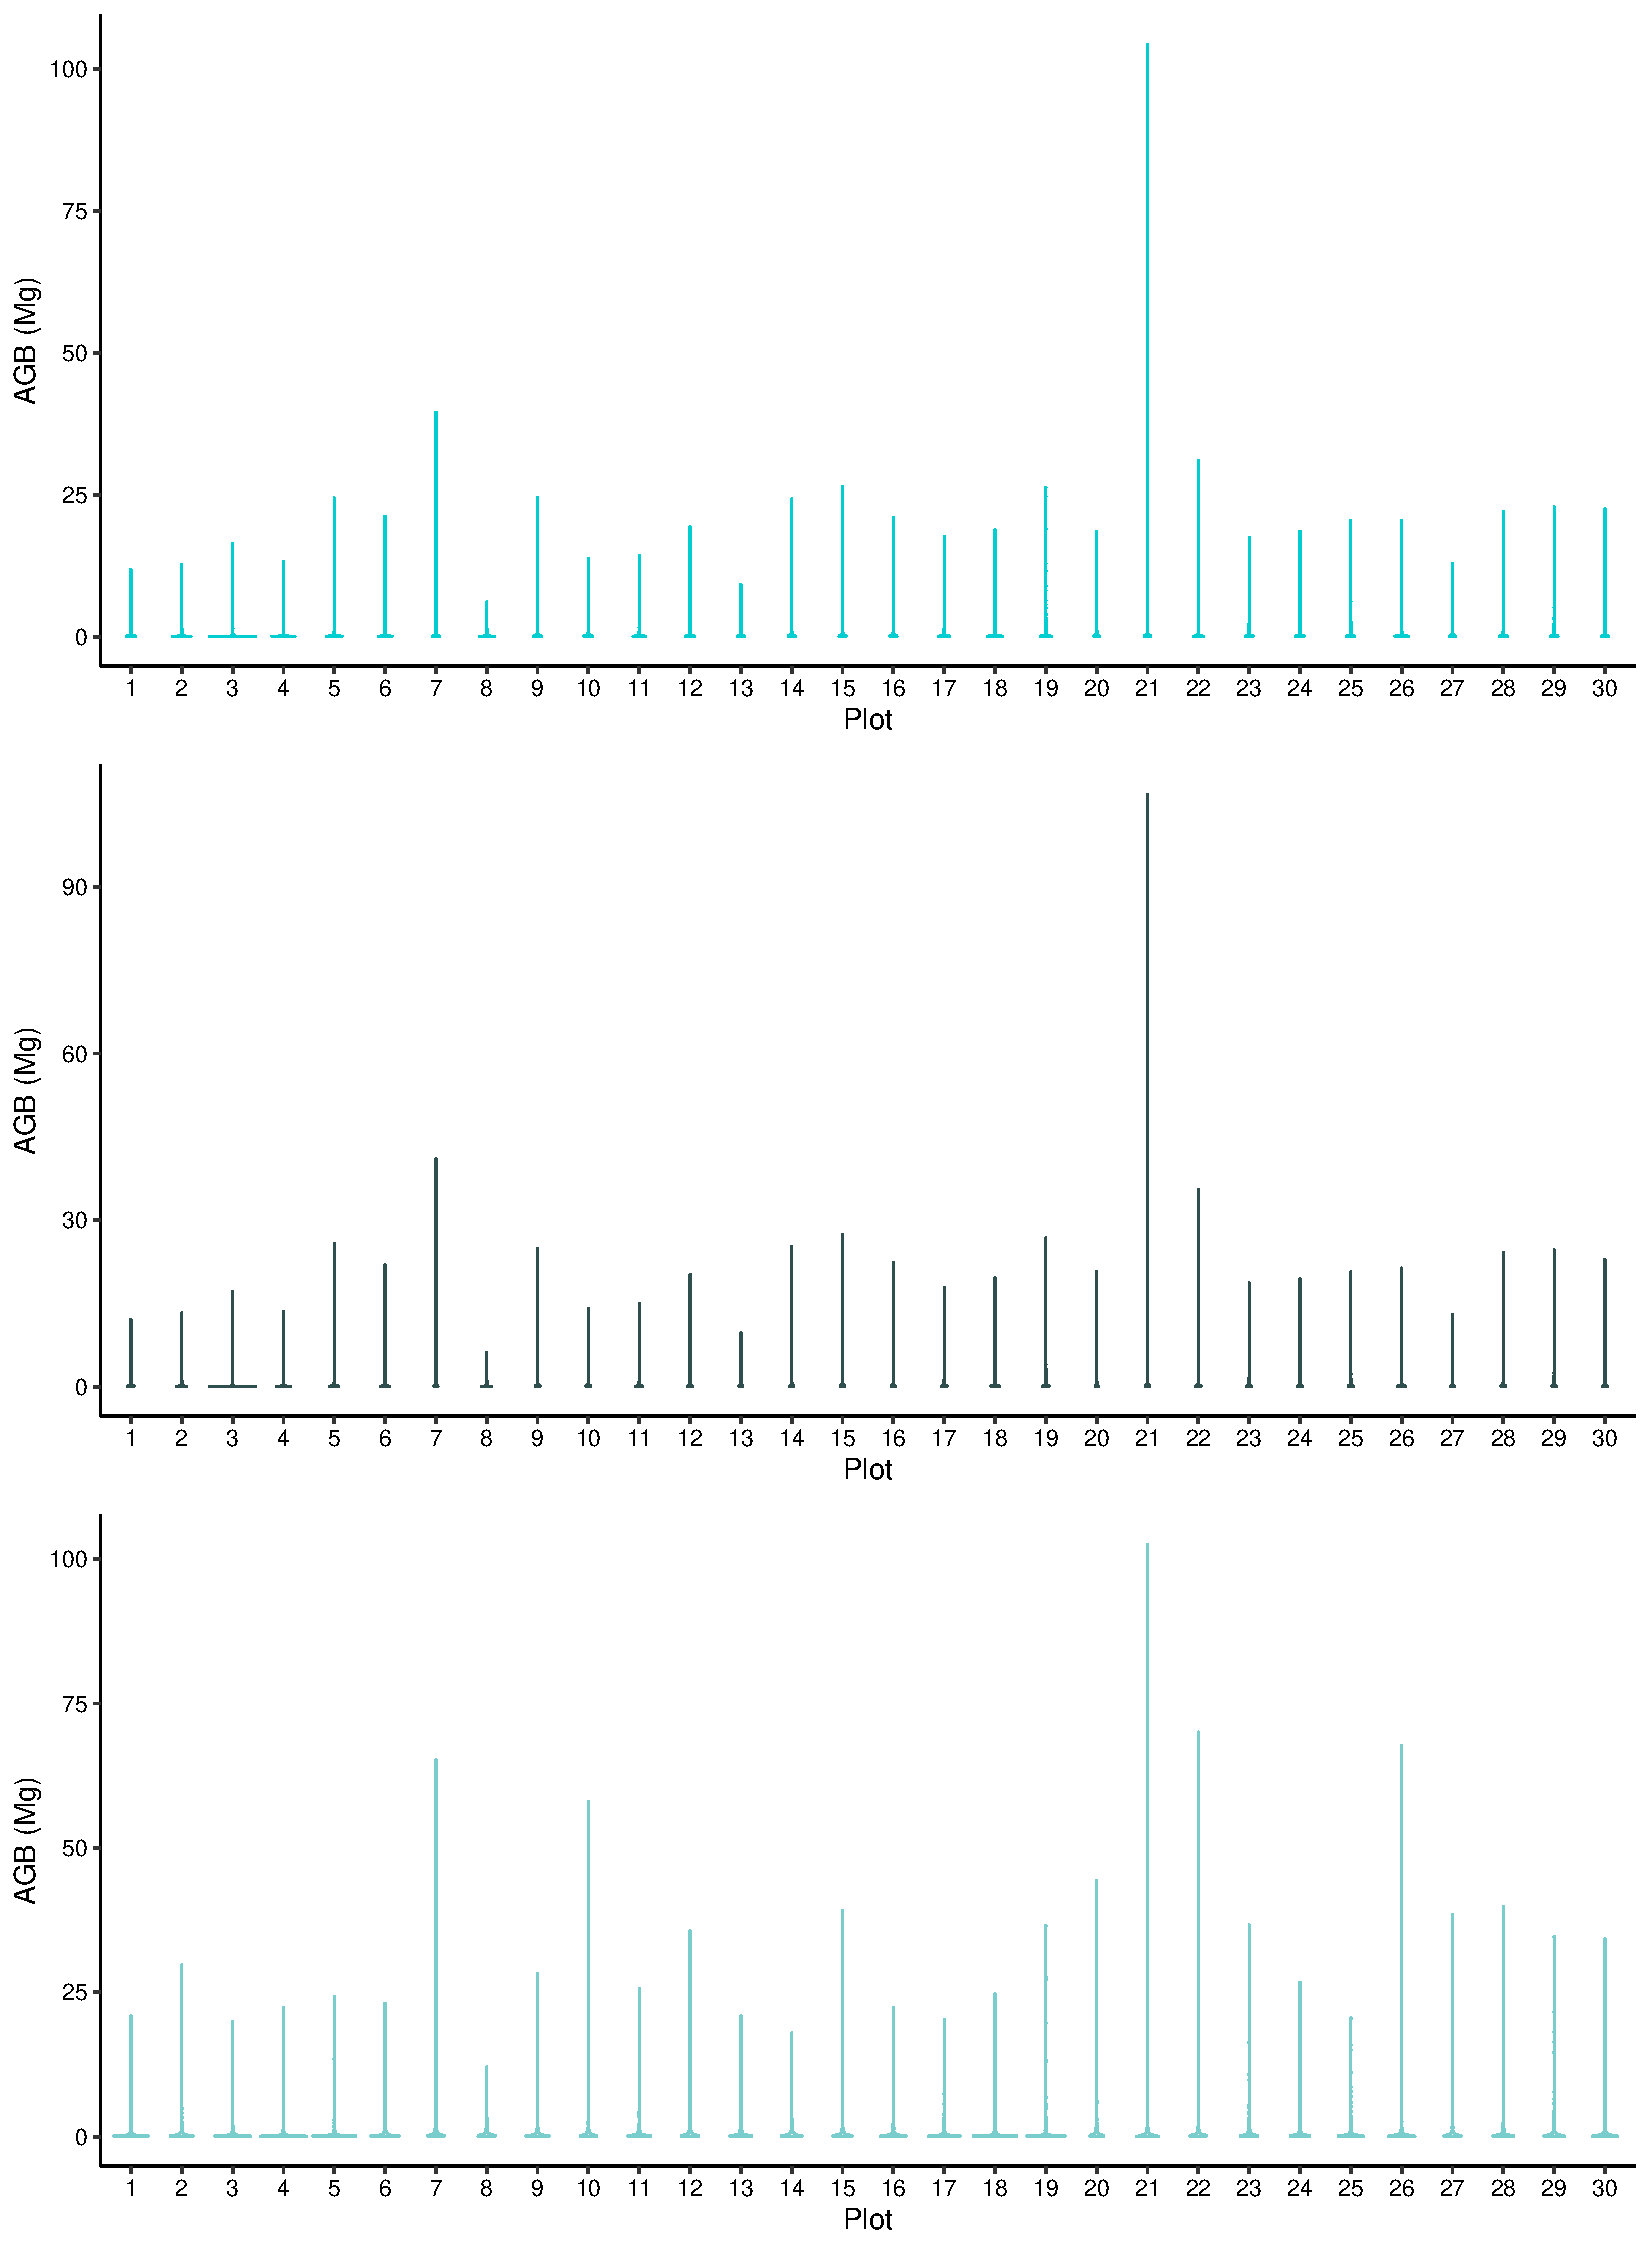
\includegraphics{Project_Template_files/figure-latex/dataviz_2013-1.pdf}
\caption{Relationship between above ground biomass at each plot in 2005,
2009, and 2013.}
\end{figure}

\newpage

Figure 4 displays the sum AGB of all trees within each plot to vizualize
the differences in AGB from one plot to another. For simplicity, the
measurements collected in 2013 were the sole focus. Here we can more
difinitively see the differences between total AGB at each plot. Where
some plots, for example plot 1, had total AGB as low as 100 Mg, plot 22
had a total AGB of over 500 Mg (Figure 4). These differences prompted
the second study question: what environmental variables may be affecting
the amount of total AGB within a plot.

\begin{figure}
\centering
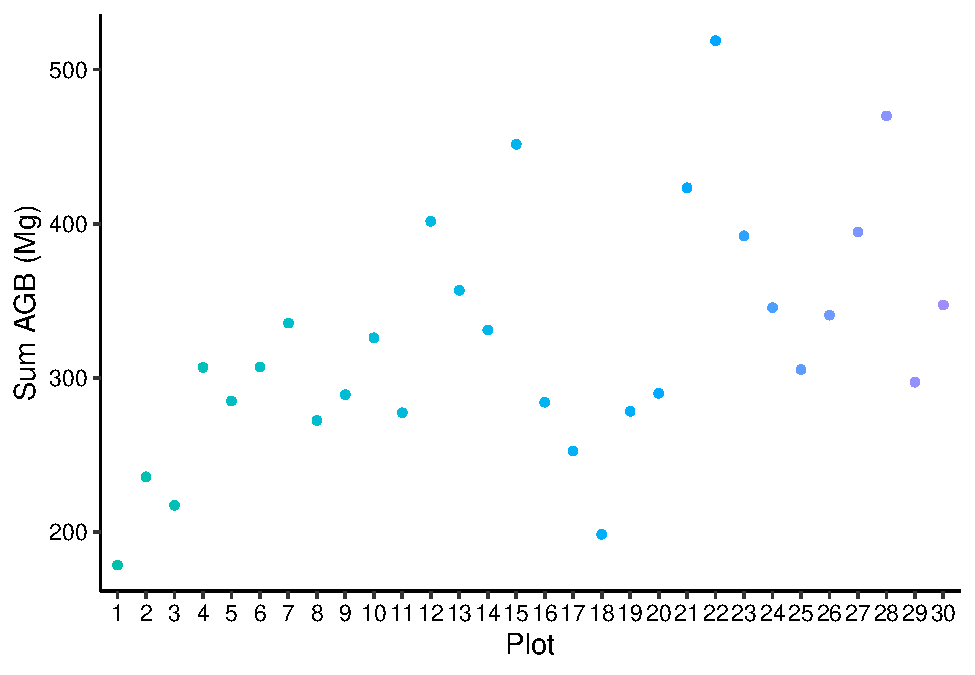
\includegraphics{Project_Template_files/figure-latex/dataviz_sum_2013-1.pdf}
\caption{Relationship between total above ground biomass at each plot in
2013.}
\end{figure}

\newpage

\begin{figure}
\centering
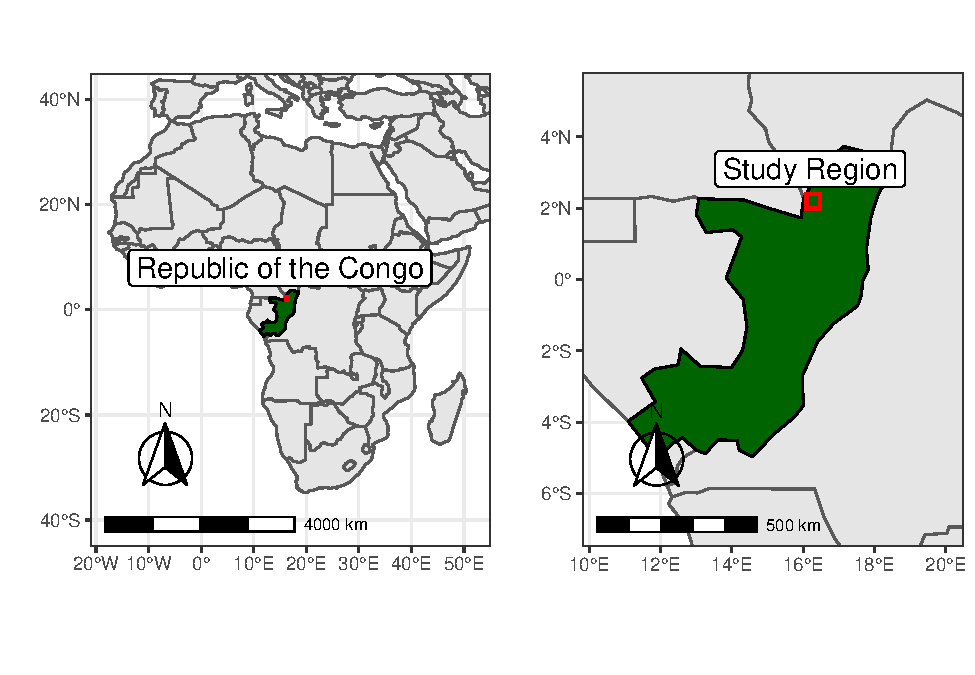
\includegraphics{Project_Template_files/figure-latex/mapping1-1.pdf}
\caption{Map displaying the location of the forest plots within the
Republic of Congo, Africa.}
\end{figure}

\begin{figure}
\centering
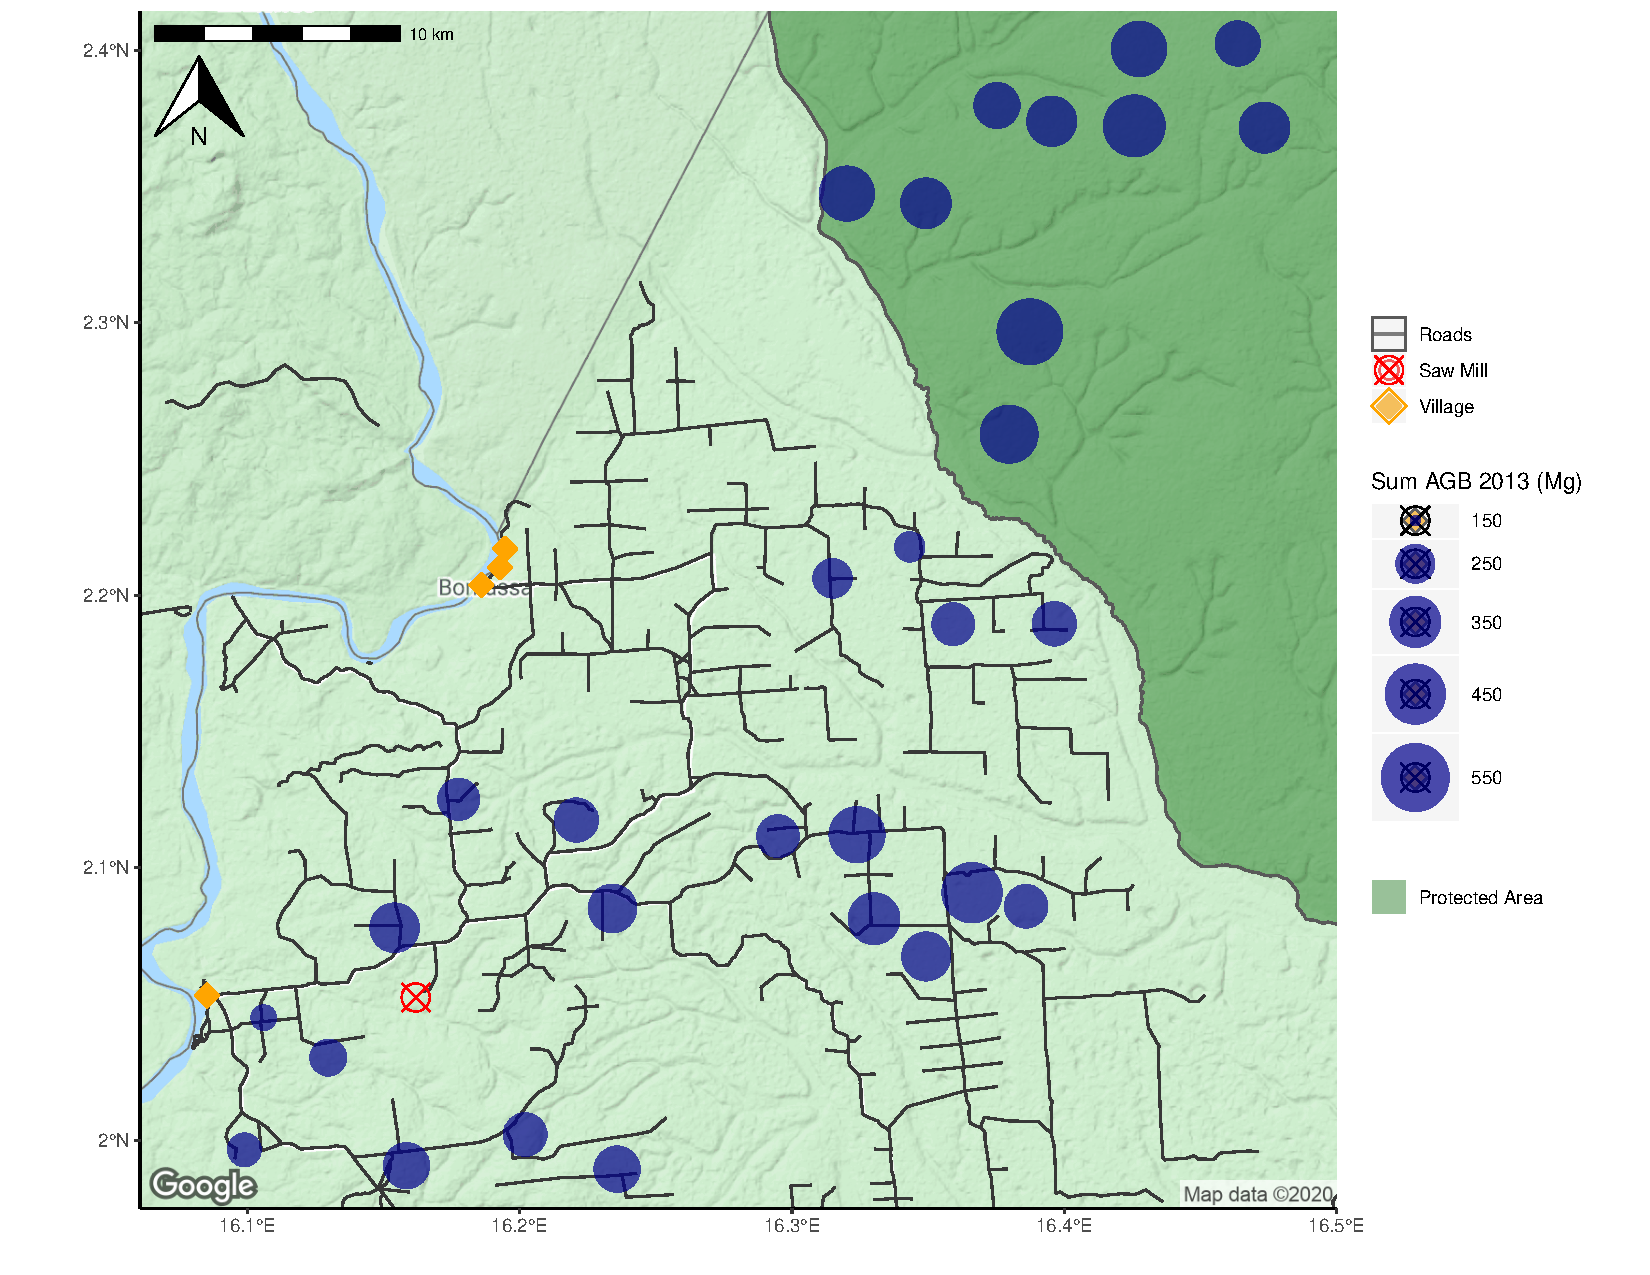
\includegraphics{Project_Template_files/figure-latex/mapping2-1.pdf}
\caption{Sum of above ground biomass (Mg) at each plot location in 2013.
Nearby road, village, saw mill, and protected area locations are plotted
to visualize the relationship between these variables and the amount of
above ground biomass.}
\end{figure}

\newpage

\hypertarget{question-1-is-there-significant-difference-in-agb-between-each-of-the-years-of-data-collection-2005-2009-and-2013}{%
\subsection{Question 1: Is there significant difference in AGB between
each of the years of data collection (2005, 2009, and
2013)?}\label{question-1-is-there-significant-difference-in-agb-between-each-of-the-years-of-data-collection-2005-2009-and-2013}}

In order to determine if there is significant increases in AGB between
the years of data collection, a one-way anova was utilized to assess the
effect that year has on the amount of AGB. A post-hoc Tukey test was
implemented on the anova model to determine if there were significant
differences between AGB for each year compared to the others.

\textbf{The results show that there was a significant increase in AGB
from 2005 to 2013, however not from 2005 to 2009 (ANOVA,
p\textless{}0.001, F2,32750 = 42.6). The Tukey test reveals that there
is no significant difference between the AGB values in 2005 compared to
2009 (p=0.287), whereas there is a significant difference between total
AGB in 2005 and 2013 (p \textless{} 0.001) and between 2009 and 2013 (p
\textless{} 0.001).}

\hypertarget{question-2-which-environmental-factors-are-significant-predictors-of-agb}{%
\subsection{Question 2: Which environmental factors are significant
predictors of
AGB?}\label{question-2-which-environmental-factors-are-significant-predictors-of-agb}}

In order to determine which variables significantly impact amount of AGB
at a plot, a generalized linear model was implemented. For simplicity,
only data from 2013 were analyzed. In this model, HFI, GlobCover, soil
type, precipitation sum, distance to road, distance to village, distance
to protected areas, and distance to saw mills were all considered as the
predictor variables, and sum of AGB was the response variable. The step
function was implemented to determine the best model by testing the
different combination of predictor variables with the response variable,
and designating the model with the lowest Akaike's Information Criterion
(AIC) value. The model with the best fit included precipitation,
distance to road, distance to village, distance to protected area, and
distance to saw mills as predictor variables. Of these variables, all of
them apart from distance to roads represented statistically significant
impacts on change in AGB.

\textbf{The results of this model show that AGB increased with
increasing precipitation, distances further from roads and villages, and
distances closer to saw mills and protected areas (linear regression, R2
= 0.31, df = 5,24, p = 0.01)} (Figure 7)

\newpage

Figure 7 shows that the model fits the data well. The QQplot displays
that the data are not normal. The Residuals vs Fitted and the
Scale-Location graph show that the data are not gathered strongly to
either side, and are evenly distributed around the line. Finally, the
Residual's vs Leverage plot shows that the points are all within Cook's
Distance, thus there are no drastic outliers.

\begin{figure}
\centering
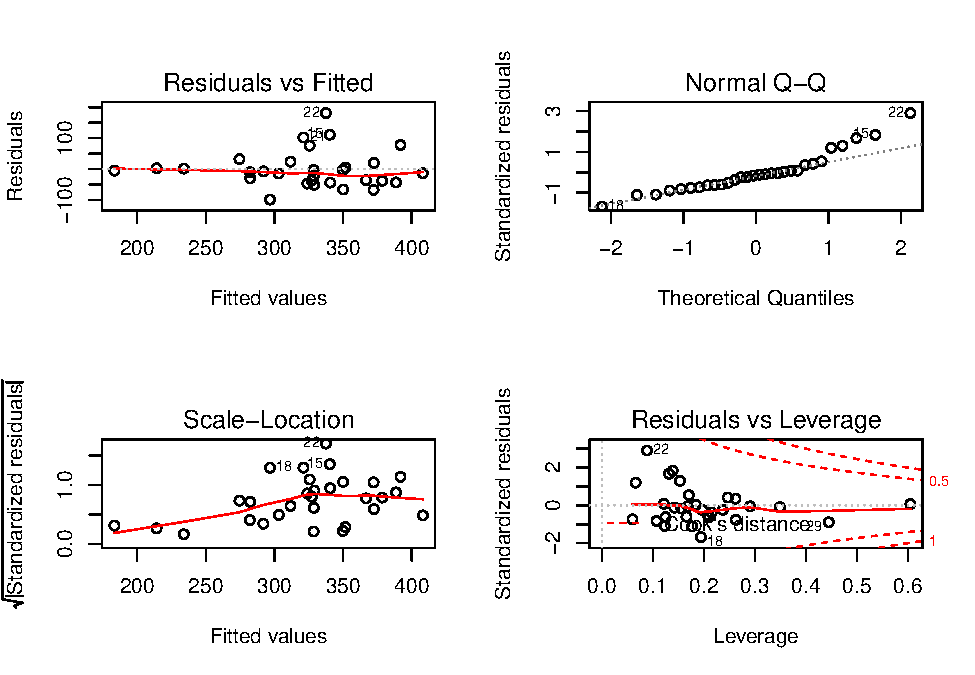
\includegraphics{Project_Template_files/figure-latex/modelfit-1.pdf}
\caption{Fit of the model that represents the effect of total
precipitation, distance to the nearest road, distance to the nearest
village, distance to the nearest protected area, and distance to the
nearest saw mill on total AGB at the plots in 2013}
\end{figure}

\newpage

\hypertarget{summary-and-conclusions}{%
\section{Summary and Conclusions}\label{summary-and-conclusions}}

Overall, this study found that there was no significant increase in
total AGB across all plots between 2005 and 2009. However, there was a
significant increase from 2005 to 2013, and from 2009 to 2013. This is
not what one would expect to find in an undisturbed area, given that
trees continue to grow with time. However, it is possible that the rate
of logging exceeded the rate of tree growth between the years 2005 and
2009. Further research would have to be done to determine the cause of
this lack of AGB increase. This study also found that precipitation,
distance to villages, distance to protected areas, and distance to saw
mills all had a significant impact on the amount of AGB within a plot.
AGB increased with increasing precipitation and increasing distance from
the villages. AGB also increased in plots that were closer, or were
located within the protected area. This all logically makes sense, given
that rainfall increases tree growth, and the unprotected plots that are
closer to villages are at an increased risk of logging. However, we did
not expect to find that AGB would increase the closer the distance to
the saw mill. It is clear from the lack of AGB increase from 2005 to
2009 and from the inverse relationship between AGB and distance to saw
mills that further analysis is needed to explain some of these
unexpected results. One possible source of error is the blank tree
measurements in the data mentioned early in this report, or it is
possible that illegal or legal logging is occurring at unprecedented
rates. If the latter is true, studies like these have the potential to
bring awareness to practices that cause hard to the environment, and
could impact the

\newpage

\hypertarget{references}{%
\section{References}\label{references}}

Chave, J., Réjou-Méchain, M., Búrquez, A., Chidumayo, E., Colgan, M. S.,
Delitti, W. B., \ldots{} Vieilledent, G. (2014). Improved allometric
models to estimate the aboveground biomass of tropical trees. Global
Change Biology, 20(10), 3177--3190. doi: 10.1111/gcb.12629

Duncanson, L., Armston, J., Disney, M. et al.~The Importance of
Consistent Global Forest Aboveground Biomass Product Validation. Surv
Geophys 40, 979--999 (2019).
\url{https://doi.org/10.1007/s10712-019-09538-8}

\end{document}
